\documentclass[All.tex]{subfiles}
%%---------------------------%
%%---- Обычный файл      ----%
%%---------------------------%
%\sloppy
%\documentclass[14pt,a4paper,oneside]{extarticle}	% Размер основного шрифта и формата листа
%\usepackage{xltxtra}						% Используется для вывода логотипа XeLaTeX
%\usepackage{xunicode}						% Кодировка документа
%\usepackage{polyglossia}					% Загружает пакет многоязыковой верстки
%\newfontfamily\russianfont{Book Antiqua}
%%\setmainfont{Liberation Serif}						% Основной шрифт текста
%\setmainfont{Book Antiqua}
%\setdefaultlanguage{russian}				% Основной язык текста
%\setotherlanguage{english}					% Дополнительный язык текста
%\linespread{1}							% Межстрочный интервал выбран полуторным
%\usepackage[left=2.5cm,
%right=1.5cm,vmargin=2.5cm]{geometry} % Отступы по краям листа
%\bibliographystyle{ugost2008}
%
%\usepackage{xcolor}
%\usepackage{hyperref}
%% Цвета для гиперссылок
%\definecolor{linkcolor}{HTML}{359B08} % цвет ссылок
%\definecolor{urlcolor}{HTML}{799B03} % цвет гиперссылок
%\hypersetup{pdfstartview=FitH,  linkcolor=linkcolor,urlcolor=urlcolor, colorlinks=true}
%
%%---------------------------%
%%---- Пакеты расширений ----%
%%---------------------------%
%\usepackage{xcolor}
%\usepackage{hyperref}
%% Цвета для гиперссылок
%\definecolor{linkcolor}{HTML}{359B08} % цвет ссылок
%\definecolor{urlcolor}{HTML}{799B03} % цвет гиперссылок
%\hypersetup{pdfstartview=FitH,  linkcolor=linkcolor,urlcolor=urlcolor, colorlinks=true}
%
%
%\usepackage{verbatim,indentfirst}
%\usepackage{cite,enumerate,float}
%\usepackage{amsmath,amssymb,amsthm,amsfonts}
%
%%---------------------------%
%%--- Вставка иллюстраций ---%
%%---------------------------%
%\usepackage{graphicx}
%\usepackage{subfigure}
%%\graphicspath{{Images/}}
%\usepackage{fontspec}

\begin{document}
%	\pagestyle{empty} %  выключаенм нумерацию
%\setcounter{page}{3}% Нумерация начинается с третьей страницы
%\renewcommand{\contentsname}{\center{Содержание}}
%\tableofcontents

	%\addcontentsline{toc}{section}{Опыт 9. Закон Гука}
	\section{Изгиб}


\begin{figure}[H] 
	\centering 
	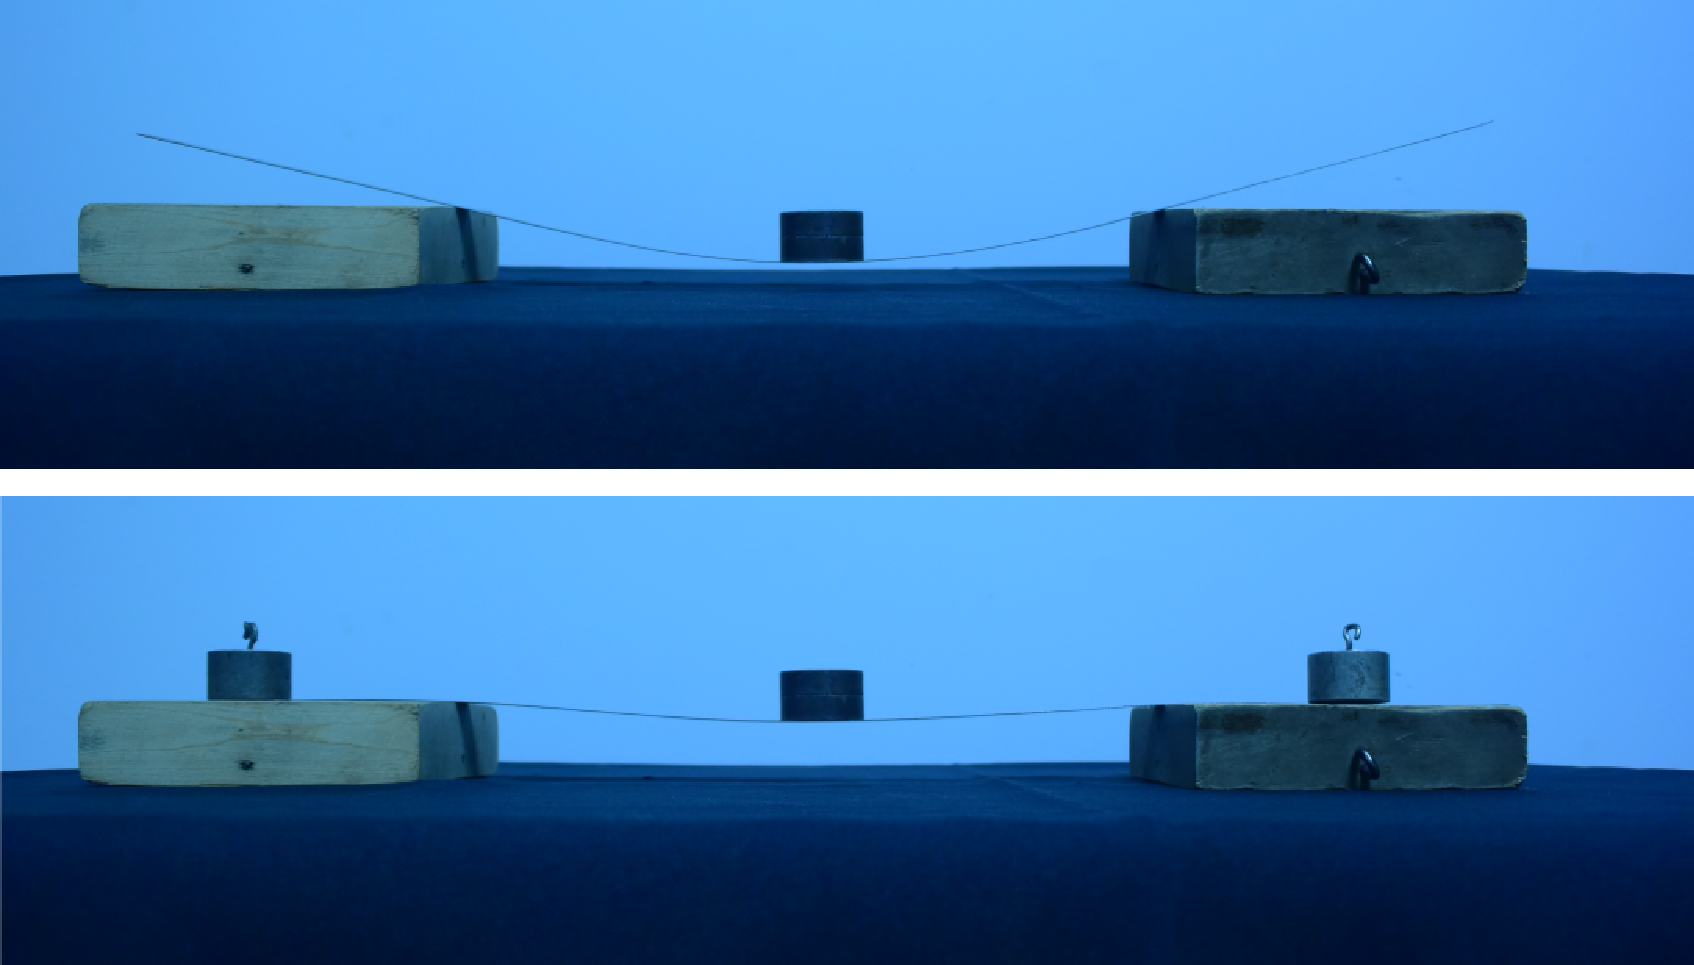
\includegraphics[width=0.9\linewidth]{bend-1.png}
	\caption{Демонстрация упругих свойств твердых тел}
	\label{bend-1}
\end{figure}

\subsection*{\textcolor{PineGreen}{Оборудование}}

\begin{enumerate}
	\item Три груза массой по 100 г каждый
	\item Узкая стальная пластинка на деревянных опорах
\end{enumerate}

\subsection*{\textcolor{PineGreen}{Основные определения и краткое описание}}

Силы упругости возникают между телами только в том случае, если тела деформированы.
Силы упругости определяются деформацией, причем по мере увеличения деформации растут и силы упругости.
Ответить на вопрос о происхождении деформаций можно, только зная законы движения.
Деформации возникают потому, что различные части тела движутся по-разному.

Подобно пружине, всякое другое тело, опирающееся на подставку или укрепленное на подвесе, оказывается соответственно сжатым или растянутым.
Именно потому, что тело оказывается деформированным, оно действует с определенной силой на подставку или подвес.
На подставку или подвес действует не сила тяжести (эта сила действует на самое тело), а сила, обсуловленная деформацией тела; эту силу называют весом.
Сила тяжести является лишь причиной возникновения деформаций.

\subsection*{\textcolor{PineGreen}{Теория}}

Вместе с самим телом оказывается деформированной и подставка, на которой тело лежит (рис.\ref{bend-2}), или подвес, на котором оно висит.
Сила, действующая на тело со стороны подставки или подвеса, - это сила упругости со стороны деформированных подставки или подвеса.
\begin{figure}[H] 
	\centering 	
	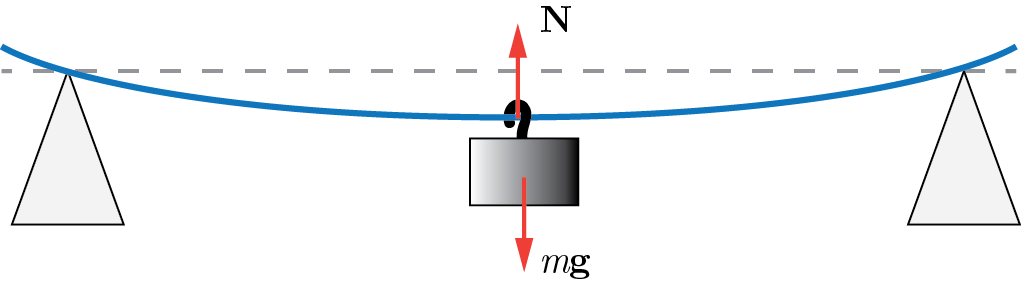
\includegraphics[width=0.75\linewidth]{bend-2.png}
	\caption{Прогиб опоры}
	\label{bend-2}
\end{figure}

Тело оказывается в равновесии под действием этой силы упругости или силы тяжести, на него действующей.
Каждая часть тела также находится в равновесии под действием силы тяжести и упругих сил, действующих на данную часть тела со стороны прилегающих к ней частей тела.



\end{document}